\documentclass[10pt,a5paper,twoside]{article}
\usepackage{coling2012}
\title{Distant supervision learning of DBPedia relations}
\author{}
%\author{$Marcin~Zaj$ą$c^{1, 2}~~~Adam~Przepi$ó$rkowski^{1, 2}$\\
%{\small (1) Institute of Computer Science, Polish Academy of Sciences\\ 
% 		(2) University of Warsaw\\
%  \texttt{marcin.zajac@students.mimuw.edu.pl, adamp@ipipan.waw.pl} \\ 
%}}

\hypersetup{
   colorlinks=false,
   pdfborder= 0 0 0
}

\begin{document}
\maketitle
\abstractEn{
This paper presents DBPedia-extender, an information extraction system that aims at extending an existing ontology of geographical entities by extracting information from text. The system uses distant supervision – training data is constructed based on matches between values from infoboxes (taken from DBPedia) and Wikipedia articles. For every relevant relation, a sentence classifier and a value extractor is trained. The sentence classifier selects sentences expressing a given relation and the value extractor extracts values from selected sentences. The results of manual evaluation on a few selected relations are reported.
}
\abstractOL{
\\\\
{\centering{{\Large{\textbf{Uczenie ze słabym nadzorem relacji z DBPedii (in Polish)}}}}}\\\\
W artykule przedstawiano DBPedia-extender, system ekstrahujący informacje, który ma na celu rozszerzenie istniejącej ontologii obiektów geograficznych poprzez wydobywanie informacji z tekstu. System korzysta z metody uczenia ze słabym nadzorem – dane treningowe są konstruowane na podstawie zgodności pomiędzy wartościami z~infoboksów (branymi z DBPedii) i~artykułów z~Wikipedii. Dla każdej istotnej relacji trenowany jest klasyfikator zdań i~ekstraktor wartości. Klasyfikator zdań wybiera zdania wyrażajace daną relację, a~ekstraktor wydobywa wartości z wybranych zdań. W pracy przestawione są wyniki ręcznej ewaluacji przeprowadzonej na kilku wybranych relacjach.
}
\keywordsOL
{information extraction, distant supervision learning, ontology construction, DBPedia, Wikipedia}
{ekstrakcja informacji, uczenie ze słabym nadzorem, budowanie ontologii, DBPedia, Wikipedia}

\newpage
\section{Introduction}
\subsection{Wikipedia and DBPedia}
Wikipedia is a free and multilingual Internet encyclopedia edited by thousands of users. Its English, most popular version has currently over 4 million articles. Wikipedia articles are a very useful resource for natural language processing. Unfortunately, Wikipedia in itself lacks many features useful in information extraction. It supports only keyword-based search and does not allow the user to ask most sophisticated questions, for example to return all European countries with more than a million inhabitants or to return all geographic entities in a given radius from a specified location. However, the necessary information to answer such queries is present in Wikipedia in the form of infoboxes. An infobox is a list of attribute, value pairs describing the most important facts about an entity. For example an infobox for a country would contain, among others, information about its capital, population, area and currency.

DBPedia is a free ontology created by processing Wikipedia infoboxes. Building an ontology from infoboxes is a difficult task, because the same concept may be expressed using different names, for example birthplace and place of birth. DBPedia, with help from contributors, developed a mapping from different infobox properties into an ontology, which helps reduce synonyms into single concepts. The extraction algorithm is described in detail in \cite{al2007}. DBPedia uses the Resource Description Framework (RDF) to represent the extracted information and a SQL-like SPARQL query language to enable querying the data. As of August 2012, the English version of the ontology contains 3.77 million entities, out of which 573,000 are classified as places (including 387,000 populated places). DBPedia, like Wikipedia, has multiple language versions.

\subsection{Goal}
Most Wikipedia articles do not have infoboxes and existing infoboxes are often incomplete, which means that DBPedia contains only a fraction of information contained in Wikipedia. The goal of the current work is to extend the DBPedia ontology by extracting relations from Wikipedia free text (see Figure 1).

\begin{figure}[htbp] 
\begin{center}
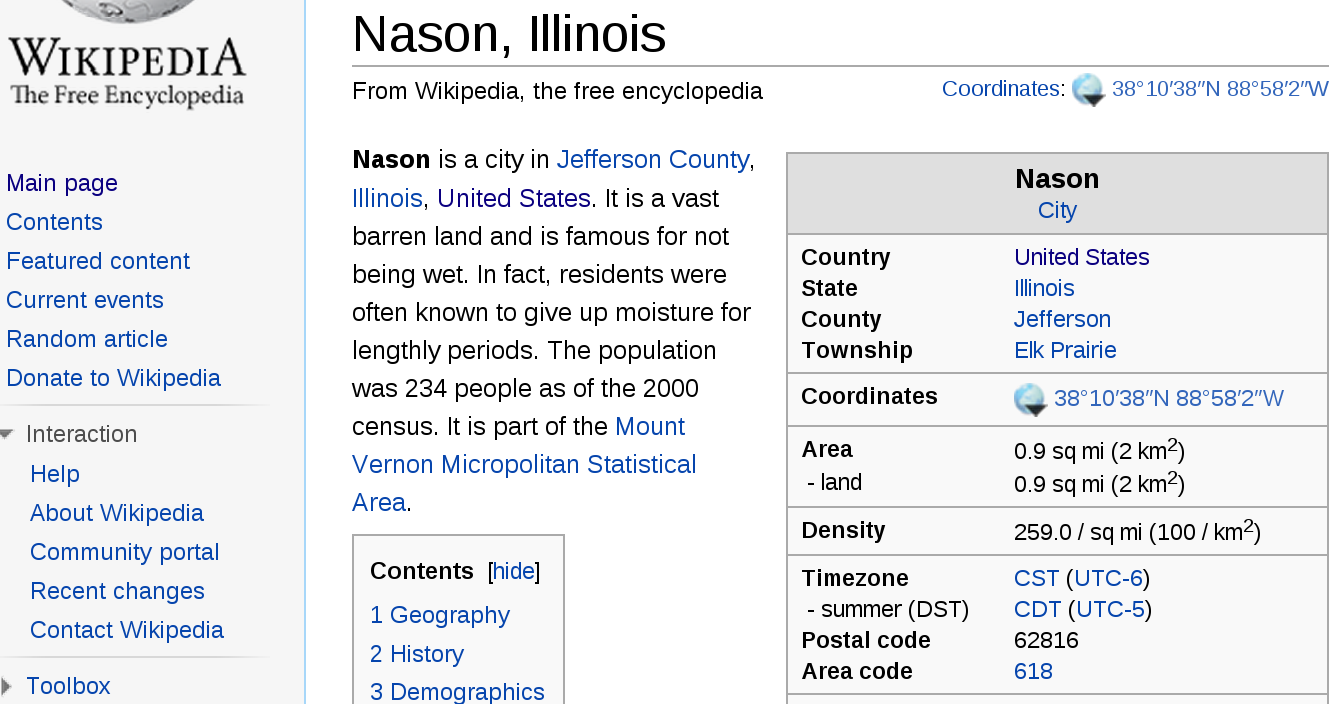
\includegraphics[scale=0.29]{nason.png}
\caption{Illustration of the aim of the developed system. The article has an infobox, but the value of population is absent from it. However, the fact that the city has 234 inhabitants is expressed in the text. The system is expected to be able to extract that information.}
\end{center} 
\end{figure}

\section{Related work}
The distant supervision method of constructing training data adopted in this paper was first presented in \cite{ww2007}. The authors developed Kylin, a system that creates new infoboxes or completes existing ones by extracting information from Wikipedia text. They evaluated their results on a few types of infoboxes. They achieved precision ranging from 74\% to 97\% and recall ranging from 60\% to 96\%. In \cite{ww2010} they showed that they managed to improve their results by using dependency parsing.

\cite{lbn2010} describes a system called iPopulator, which automatically populates infoboxes of Wikipedia articles. Like Kylin, it was tested on whole infoboxes, achieving a precision of 91\% and recall of 66\%. 

In contrast, the system presented in this paper was evaluated on selected relations, enabling us to analyze in detail differences in performance among them. Two types of relations are identified, for which performance differs significantly – numerical relations are generally easier to extract than textual ones.

Unfortunately, the different approach in evaluation makes it difficult to compare results achieved by our system with those shown in papers cited above.

\section{Extraction algorithm}
The system uses distant supervision learning algorithm to learn new <subject, relation, object> triples. It trains a classifier and an extractor for every relation. The classifier predicts if a given sentence expresses the relation. The extractor tries to extract the value of the relation from sentences selected by the classifier.

\subsection{Preprocessing}
Before models are trained, some preprocessing of the Wikipedia articles is necessary.
\begin{compactitem}
    \item Conversion to a plain text corpus – Wikipedia articles are written in Wikitext markup language which must be stripped before any natural language processing can be started.
    \item Sentence detection and tokenization.
    \item Retokenization of geographic names – the tokenizer splits multi-part names into separate tokens. The process is reverted by joining geographic names so that they constitute a single segment. DBPedia was used as a source of geographic entities.
    \item Conversion of geographic names into their most often used form ("United States of America" and "the U.S." become "United States"). Wikipedia redirect links are used as a source of synonyms.
\end{compactitem}

\subsection{Constructing training data}
Training data is constructed separately for every relation. At first all <subject, object> pairs that are in a given relation in DBPedia are retrieved. Then articles about each of the subjects are processed. In the articles, the system looks for sentences that contain the value of the object. If there is a single such sentence in the article, the sentence and the value are simply used as training data. If the value occurs in more than one sentence, only sentences that contain at least a part of the name of the relation are used.

For example, if the relation name is "populationTotal", a sentence "X has population of Y" will be selected if Y matches, but sentence "X has Y inhabitants" will not be selected, despite the fact that it expresses the relation. On the other hand, sometimes a sentence that should not be selected, will be. For example if Y is a capital of X, but a sentence "Y is the biggest city in X." is the only sentence referring to Y, the sentence will be selected, despite the fact that it does not express the fact that Y is the capital of X.

The data constructed this way is very imbalanced because a vast majority of sentences are negative examples. Because the classifier used is designed to maximize accuracy it may predict the majority class much more often than the minority class. To avoid that problem undersampling is performed – randomly selected negative examples are removed, so that in the end there is the same number of positive and negative training examples. 

In future versions of the system, it might be a good idea to try a different approach to solving that problem. One approach would be to use a cost-sensitive classifier, which is discouraged from selecting the majority class by a change in misclassification costs. Balanced random forest classifiers are also known for working well with imbalanced datasets.

\subsection{Selecting candidates for learning}
The system tries to extract relations expressed in Wikipedia, but not present in DBPedia. However, applying the presented algorithm to every Wikipedia article would take too much time and would probably result in lowered precision. Therefore, it is necessary to develop a method of selecting entities that are suspected to be in a given relation. A simple heuristic is used, making use of the fact that every DBPedia entity has numerous types associated with it. For example Berlin is, among others, a city, a populated place and a settlement.

The system considers only those entities that have the same type as a vast majority of entities that already are in a relation. For example one can see that most entities that have a value of population are populated places. Therefore when trying to learn new values of population, only entities that are populated places can be considered. Unfortunately, this algorithm will omit some articles that contain sentences expressing the relation, because not every entity in DBPedia has a correct type.

\subsection{Sentence classifier}
The sentence classifier tries to predict if a given sentence expresses a given relation. It is a binary, yes-or-no classifier.
Support vector machine with simple features such as a set of tokens from the sentence are used. The tokens are lemmatized beforehand, stop words and rarely occurring words are removed.

\subsection{Value extractor}
The value extractor tries to extract a value from a sentence returned by the sentence classifier. Sometimes there will be no value to extract, sometimes there will be more than one. This problem can be seen as a tagging problem, where all tokens in a sentence should be labeled as positive (indicating that this is a value to extract) or negative. Conditional random fields are a natural choice for this task. The extractor uses features from a window of 3 tokens to the left and to the right. 

Following features are used by the extractor:
\begin{compactitem}
    \item the token itself,
    \item stemmed token,
    \item the position of the token in the sentence,
    \item whether all of its parts start with a capital letter,
    \item whether it is an integer or a numerical value,
    \item whether it is likely a year (between 1000 and 2012),
    \item whether it is likely a recent year (between 1990 and 2012),
    \item information about type (if the entity is present in DBPedia).
\end{compactitem}
Information about type in stored in a binary vector indicating the type of a given entity. For geographic entities, 21 relevant types from DBPedia are considered: Place, PopulatedPlace, Settlement, Country, AdministrativeRegion, Continent, Island, City, River, BodyOfWater, Stream, Lake, NaturalPlace, MountainRange, Valley, Volcano, Cave, ArchitecturalStructure, Infrastructure, Park and Building.

\section{Evaluation}
The system was evaluated on 3 relations using human labeling. For each relation, 50 geographic entities that were in a given relation in DBPedia were randomly selected. Then a human annotator selected values which, in his opinion, were expressed in a corresponding Wikipedia article. In some cases more than one value was thought to be expressed for one entity. In such cases, the system is said to work correctly if at least one of the values is extracted.

Note that evaluation is complicated by the fact that some relations expressed in text are often not entirely true or false. For example, when extracting a value of population for an existing city, selecting a value recorded a hundred years ago would be a mistake, but finding a value recorded in the last few years would count as a success. The cases that lie between these two extremes are disputable. On the other hand, if an article about a city abandoned in the 19th century is processed, extracting a value from a distant past might not be a mistake.

Table 1 shows how many articles were processed during training and, according to the human annotator, how many of the 50 articles selected for evaluation had at least one sentence expressing the relation. All training data available was used unless there were more than 10000 articles.
\begin{table}[!h]
\setcounter{table}{0}
\centering
\begin{tabular}{ | c | c | c | }
    \hline
    relation & no. training articles & no. articles expressing relation \\ \hline \hline
    capital & 952 & 43 out of 50 \\ \hline
    river mouth & 3171 & 44 out of 50\\ \hline
    population & 10000 & 27 out of 50 \\ \hline
\end{tabular}
\caption{The number of articles used during training and the fraction of articles expressing the relation.}
\end{table}

Three results for every relation are presented: sentence classifier performance, value extractor performance and overall performance. Sentence classifier is said to work correctly if it selects at least one sentence that contains the value to be extracted. In other words, it means that the extractor has a chance of extracting the right value. Value extractor and overall performance indicate if the right value was extracted. They differ in the fact that value extractor performance does not take into account entities for which no sentence was selected by the sentence classifier.

It became clear from the start that two types of relation can be separated:
\begin{compactitem}
    \item textual (e.g. capital, country, mountain range, river mouth)
    \item numerical (e.g. total population, total area, elevation)
\end{compactitem}
Numerical values can be further divided into untyped (e.g. population) and typed values (e.g. elevation can be expressed either in meters or in feet).

It should be noted that the sentence classifier must have high recall, because if it rejects a sentence, value extractor will not be able to extract any value from it. Selecting a sentence which in fact does not
contain the value is less problematic. In contrast, the complete system, in order to be useful, should have high precision; recall is less important.

\subsection{Textual relations}
\subsubsection{Capital}
The results of extracting the capital relation are shown in Table 2.
\begin{table}[!h]
\centering
\begin{tabular}{ | c | c | c | c | }
    \hline
    result & precision & recall & F-measure \\ \hline \hline
    sentence classifier & 64\% & 67\% & 66\% \\ \hline
    value extractor     & 86\% & 83\% & 84\% \\ \hline
    overall             & 86\% & 56\% & 68\% \\ \hline
\end{tabular}
\caption{Results for capital.}
\end{table}

As can be seen in the table, the overall precision for this relation is high, recall is significantly lower. Low recall is caused by the relative sparsity of training data (less than a thousand entities have capitals defined) and the fact that being a capital may be expressed in numerous ways. These are some examples from articles used during evaluation:
\begin{compactitem}
    \item The center was Bitlis, which was called Baghesh.
    \item The main town and the site of its municipal council is the city of Nyborg.
    \item The administrative center became the city of Vologda.
    \item Its administrative seat is in the town of Nykøbing Falster.
    \item He built a citadel to be his capital in the small town of Kokand, thus starting the Khanate of Kokand.
\end{compactitem}

\subsubsection{River mouth}
The results of extracting the river mouth relation are shown in Table 3.
\begin{table}[!h]
\centering
\begin{tabular}{ | c | c | c | c | }
    \hline
    result & precision & recall & F-measure \\ \hline \hline
    sentence classifier & 64\% & 64\% & 64\% \\ \hline
    value extractor     & 78\% & 89\% & 83\% \\ \hline
    overall             & 78\% & 57\% & 66\% \\ \hline
\end{tabular}
\caption{Results for river mouth.}
\end{table}

As the table above shows, similarly to the capital relation the system has reasonable overall precision, but rather low recall. Some of the errors the system made are analyzed below.
\begin{compactitem}
    \item "Waiau River (Southland) is the outflow of Lake Te Anau, flowing from it into Lake Manapouri 10 kilometres to the south, and from there flows south for 70 kilometres before reaching the Foveaux Strait eight kilometres south of Tuatapere."\\ Foveaux Strait is the value that should be selected, but the system extracts Lake Manapouri into which the river flows, but it also flows out of it, which means the lake is not a mouth. The distinction however is not instantly clear even for a human and is too subtle for the approach presented.
    \item "The Neva River is a river in northwestern Russia flowing from Lake Ladoga through the western part of Leningrad Oblast (historical region of Ingria) to the Neva Bay of the Gulf of Finland."\\ Neva Bay should be selected, however it is not recognised as a geographic entity, because it has no type defined in DBPedia.
    \item "Later, the river Barduelva joins it [Målselva]."\\ The system extracts Barduelva as the mouth of Målselva, however it should extract the reverse relation – Målselva is the mouth of Barduelva. The value extractor is unable to distinguish between these two cases.
\end{compactitem}

Generally, textual relations have reasonable precision, but rather low recall. This is partly caused by the fact that many entities are not recognised as such, because they do not have a correct type in DBPedia. It seems a good idea to use a additional named entities lexicon for named entity recognition.

\subsection{Numerical relations}
\subsubsection{Total population}
The results of extracting the total population relation are shown in Table 4.
\begin{table}[!h]
\centering
\begin{tabular}{ | c | c | c | c | }
    \hline
    result & precision & recall & F-measure \\ \hline \hline
    sentence classifier & 62\% & 96\% & 75\% \\ \hline
    value extractor     & 81\% & 100\% & 90\% \\ \hline
    overall             & 81\% & 96\% & 88\% \\ \hline
\end{tabular}
\caption{Results for total population.}
\end{table}

As can be seen in the table, overall recall is very high, only one value is not extracted. The value is not found because the classifier rejected the sentence "It has around 8200 residents and is situated in the Forest Heath district of Suffolk close to the county boundaries of both Norfolk and Cambridgeshire and at the meeting point of the The Fens and the Breckland natural environments." This example shows that the sentence classifier has problems with correctly classifying very long sentences which, apart from expressing the relation, contain other information.

Precision is lowered by two types of errors. First is caused by the assumption that sentences in an article describe the entity that is the subject of the article. That is not always the case. For example, the sentence "Its seat is located in the town of Gnesta, with some 5000 inhabitants." expresses the value of population but not for Gnesta Municipality, which is the subject of the article, but for Gnesta which is its capital. To avoid these errors in the future, it might be useful to consider only sentences if the entity is the sentence's grammatical subject.

The second type of false positive occurs when a correct value of population is extracted, but from a distant past. For example in the article about Titisee-Neustadt a sentence "In 1880 the population was 50." is selected and 50 is extracted as the value of population.

\section*{Conclusions and future work}
This paper presents a system that learns new relations about geographic entities. The system is trained on automatically constructed data based on a match between values from infoboxes (taken from DBPedia) and Wikipedia articles.

Its performance is evaluated using manually labeled data. The program works best on a numerical relation achieving precision of about 80\% and recall exceeding 90\%. On textual relations it achieves similar precision, but significantly lower recall – slightly below 60\%.

There are many ways to improve performance. Some of them are indicated throughout the article. Much improvement can be gained if an additional lexicon of named entities was used. Precision can be increased at the cost of recall, if the sentence classifier performs some dependency analysis, verifying that the grammatical subject of the sentence is the topical subject of the article.

The ultimate goal of the project is to develop a similar system for Polish, where rich morphology and the correlation of grammatical cases and grammatical functions may make it possible to identify sentence subjects without deep dependency parsing.

%\section*{Acknowledgments}
%This research was funded within CESAR (CEntral and South-east europeAn Resources), a CIP ICT-PSP project (grant agreement 271022).

\bibliographystyle{apa}
\bibliography{paper}
\end{document}
